% --[Settings]---------------------------------------------------------------
\documentclass[
	11pt,
	a4paper
]{article}%{scrartcl}

\usepackage{
	graphicx,
	color,
	%charter,										% alternative Font
	url
}

\usepackage{float}
\usepackage{longtable}
\usepackage{booktabs}
\usepackage{gensymb}
\usepackage[	colorlinks=true,
		linkcolor=blue,
		]
		{hyperref}
\usepackage[fleqn]{amsmath}
\usepackage[utf8]{inputenc}
\usepackage{wrapfig}								% wrapping pictures
\usepackage{todonotes}
\usepackage{pdfpages}
\usepackage{colortbl}
\usepackage{color}
% Define user colors using the RGB model
\definecolor{dunkelgrau}{rgb}{0.8,0.8,0.8}
\usepackage[left=2cm,right=2cm,top=2cm,bottom=2cm,includeheadfoot]{geometry}

% --[Kopfzeile]-------------------------------------------------------------
%Kopf- und Fußzeile
\usepackage{fancyhdr}
\pagestyle{fancy}
\fancyhf{}

%Kopfzeile links bzw. innen
\fancyhead[L]{\textbf{Smart Sensor Network Systems}\\Software Project Plan - Group 6}
%Kopfzeile rechts bzw. außen
\fancyhead[R]{\today}
%Linie oben
\renewcommand{\headrulewidth}{0.5pt}

%Fußzeile mittig
\fancyfoot[C]{\thepage}
%Linie unten
\renewcommand{\footrulewidth}{0.5pt}

% --[Dokumentbegin]---------------------------------------------------------

\begin{document}
%\setlength{\parindent}{0pt}							% nicht automatisch einrücken

% auch subsubsection nummerieren
\setcounter{tocdepth}{3} 
\setcounter{secnumdepth}{3} 


\title{\textbf{Software Project Plan}\\
	Pond Environmental Measurement\\
	SSNS - Smart Sensor Network Systems\\
	Frankfurt University of Applied Sciences}
\author{Alexander K.,\\
	Sabrina B.,\\
	Rozana A.,\\
	Alexander V.D.}
\maketitle


\newpage
\pagenumbering{arabic}
\tableofcontents
\newpage

% ----------------------------- Introduction --------------------------------------------
\section{Introduction}
The Idea of this Project is to build a System, based on a Wireless Smart Sensor Network, to measure a ponds water Temperature and the weather conditions that influence the ponds temperature. The Data from the measurements shall be stored in some thing like a database and be visualizable on a PC. The goal is the visualization of a reliable 24/7 data aquisition.
\\\\
For the breeding and keeping of fish in a pond it is often relevant to know the ponds temperature and the range in which the temperature stays over a longer period of time. We also expect some interesting results from a system like that.

% ------------------------------- Project Specification ---------------------------------
\section{Project Specification}
\subsection{Project Description}
The System consists of the following Components:
\begin{itemize}
\item one underwater Temperature measuring Sensor Node
\item one over water weather measuring Node (Temperature, Light)
\item one indoor Node collecting and storing the measured Data, connected to ethernet
\item A PC running a visualizing Application
\end{itemize}
The sensors measure the weather conditions and pond temperature. The values get forwarded to an indoor Data Collecting Node with ethernet access. There the Data is going to be logged. Using a Computer a history of the measurements (seen as tables and graphs) can be viewed via a special application.
\\\\
The Three Nodes will communicate via the ZigBee Protocol, using XBee Modules.
\begin{figure}[h!]
  \caption{Pond Envrionmental Measurement}
  \centering
    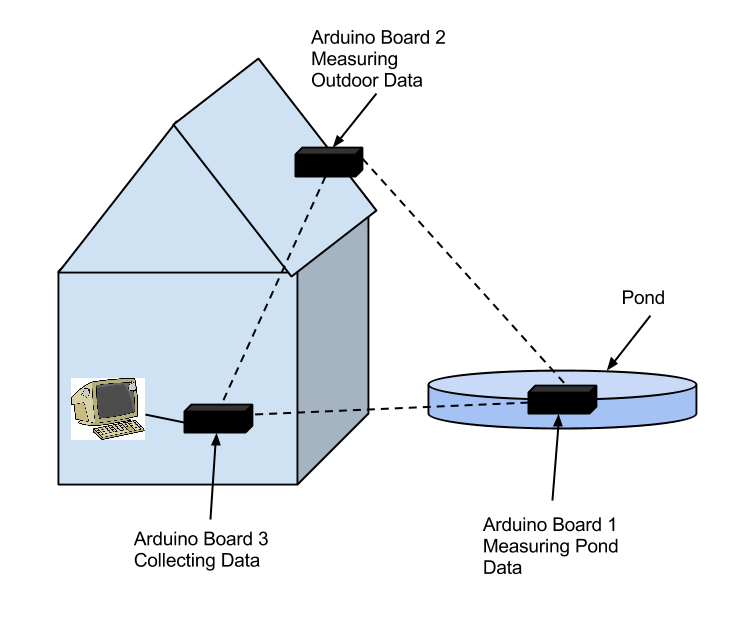
\includegraphics[width=0.50\textwidth]{../Images/ssns_project.png}
\end{figure}
\\\\
The outdoor sensor nodes are going to operate independant of a power source meaning that these Nodes will be equipped with Solar panels and batteries. They should be able to run 24 hours every day just by the power provided by the solar panel and the batteries (that get charged by the solar panel).
\\\\
In this project we want to concentrate on the Software part of the System. To build the Outdoor Nodes in a Weather Proof way and designing them independant of a Power Supply by using Solar is a complex task. Finishing the Hardware is an optional aspect of our project. We will design the necessary circuits for attaching the sensors to the arduino Nodes and use the Nodes to test our Software on. The task of building weatherproof, solar powered Nodes based on the sensor circuit design is optional or can be done in a future project.

\subsection{Process Model}
As Process Model we chose the Rational Unified Process (RUP). RUP has the advantage of being iterative and incremental while also being relatively lightweighted. All Project activities can be used any time when needed, this gives us flexibility.
\\\\
The Rational Unified Process is an Interactive software development process framework. It was created by Rational Software Corporation, a division of IBM since 2003. It enhances team productivity and creates and maintains models. It is also a guide to effectively use the Unified Modeling Language. Its goal is to deliver a high quality product that the customer actually wants.
\\\\
The RUP model is mainly used in Telecommunications, Transportation, aerospace, defense, manufacturing ,financial services and in system integrators.
\\\\
Well-defined and well-documented software development processes are key to the success of software projects. CMM(Capability Maturity Model) by the software engineering Institute (SEI) has become a beacon. Theoretical know-how fails to materialize in practice. Sometimes there is no process know-how at all. Resulting in chaos, failure and Loss. In this cases RUP can help. It is a mature, rigorous and flexible software engineering process.
\\\\
We choose RUP for our project because of its luxary features, usage of Best Practices and also for its development cycle process. The mensioned terms are explaing as follows:
\\\\
Features of RUP :
\begin{itemize}
\item Iterative Development
\item Requirements Management
\item Visual Modeling of Systems
\item Quality Management
\item Change Control Management
\end{itemize}

Compare to the traditional waterfall process, the iterative process has the following advantages:
\begin{itemize}
\item Risks mitigated ealier
\item Change is more manageable
\item Higher level of reuse
\item The project team can learn along the way
\item Better overall quality
\end{itemize}

The 6 Best Practices are as follows :
\begin{enumerate}
\item Develop software iteratively
\item Manage requirements
\item Use Component-based architechtures
\item Visually model software
\item verify software quality
\item Control changes to software
\end{enumerate}

In every Iteration, all of these tasks can be performed with a certain weight. In the first iterations a lot of weight will be on the Requirements and less on the Deployment. In later iterations Deployment is going to gain weight while the Requirements are almost done. So it is possible to react to change, and to correct errors, with the beginnig of every iteration and it will be accomplished at the end of the iteration. It is also intended that the software gains functionality with each iteration (incremental development).

All iterations of a project are grouped into 4 phases.
\begin{enumerate}
\item Inception
\item Elaboration phase
\item Construction phase
\item Transition phase
\end{enumerate}
\begin{itemize}
\item Each phase is concluded with a well-defined milestone
\item Each phase has a specific purpose
\end{itemize}
\textbf{Inception phase:}
\begin{itemize}
\item A vision document
\item An intial use-case model
\item An Initial project glossary
\item An initial business case
\item A project plan, showing phases and iterations .
\item A business model
\end{itemize}
Project milestone : The Lifecycle Objectives Milestone
\\\\
\textbf{Construction Phase:}\\\\
The construction Phase is concerned with moving from the executable architechtures created in the Elaboration phase to an operational system
\begin{itemize}
\item the focus here is to develop the application to the point where it is ready for deployment
\item Focus is on implementation of the design
\end{itemize}
Project Milestone : Initial operational Capability 
\\\\
\textbf{Elaboration Phase:}
\begin{itemize}
\item A use-case model (at least 80\% complete) supplementary requirement (non functional requirement)
\item A software architechtural description
\item An Executable architechtural prototype 
\item A revised risk list and a revised business case 
\item A development plan for the overall project 
\item An updated development case specifying the process to be used 
\item A preliminary user manual (optional)
\item Domain model
\end{itemize}
Project milestone : the Lifecycle architechture Milestone
\\\\
\textbf{Transition Phase:}
\begin{itemize}
\item "Beta testing" to validate the new system against user expectations 
\item Parallel operation with a legacy system that it is replacing 
\item Conversion of operational database
\item Training of users and maintainers 
\item roll-out the product to the marketing , distribution , and sales team 
\end{itemize}
Project milestone : The product Release Milestone
\\\\
\textbf{Pros of RUP:}
\begin{itemize}
\item Regular feedback from and stakeholders
\item efficient use of resources
\item we can deliver exactly what the customer wants
\item Issues are discovered early in your project
\item Supports iterative development
\item Improved risk management
\end{itemize}\textbf{Cons Of RUP:}
\begin{itemize}
\item The process may be too complex to implement .
\item Development can get out of control
\item It is a heavyweight process
\item You need an expert to fully adopt this process
\end{itemize}


\subsection{Requirements}
\subsubsection{General Requirements}
There are Three (Software) components to be developed:
\begin{itemize}
\item Software for the two measuring Nodes (only different in respect to the sensor configuration)
\item Software for the collecting Node, with connection to Ethernet
\item PC Application for Data visualization
\end{itemize}
Ofcourse there are also Hardware components that have to be developed:
\begin{itemize}
\item Weatherproof, Solar powered water temperature measuring Node
\item Weatherproof, Solar powered weather measuring Node
\item Data colloecting Node
\end{itemize} 
When discussing the Requirements of the system it is necessary to distingush the components and to distingush the requirements for the Software from the requirements to the hardware.

\subsubsection{Overall System Requirements}
\begin{itemize}
\item reliable 24/7 data Aquisition
\item Data being storaged on the collecting Node (Some sort of Database)
\item Graphical visualization on the PC, reading Data from the collecting Node over Ethernet
\end{itemize}

\subsubsection{Data Measuring Nodes Requirements}
\begin{itemize}
\item Taking measures as the mean of multiple measurements over a short time period
\item Measures get taken after a demand by the collecting Node
\item Measures get stored localy until the collector acknowledges the receipt of the measure
\item Based on Arduino UNO and Wireless Protoshield with an XBee Module
\end{itemize}

Optional:
\begin{itemize}
\item Weather proof housing
\item independant from Power Supply by using Batteries and Solar
\end{itemize}

\subsubsection{Collecting Node Requirements}
\begin{itemize}
\item Coordinator Role in the ZigBee Network
\item knows Date and Time, set via NTP
\item Demands Measures from the measuring Nodes every half an hour
\item Measuring Nodes have 30 sec. time to answer before their measures get stored as unknown.
\item stores measures on SD-Card as CSV-File
\item Sends CSV-File over Ethernet on demand
\item Acts as TCP Server (On static IP Adress and fixed Port)
\item Based on a Arduino Ethernet with Wireless Protoshield and XBee Module
\end{itemize}

\subsubsection{PC Application Requirements}
\begin{itemize}
\item Developed in Java, GUI using Swing
\item Connects to the Collecting Node via IP/Ethernet
\item Connects as TCP-Client to collecting Node on its static IP-Adress and fixed Port
\item Data Visualization as Tables and Graphs
\item Selectable Timeframe for shown Data
\item Selectable Data to be shown in the same Graph (Pond Temperature, Air Temperature, Light Level)
\item Data Export as CSV File (Coma-Seperated-Values)
\end{itemize}

\newpage
% ------------------------------- System Architecture ---------------------------------
\section{System Architecture}
\subsection{Architecture}
The Hardware Architecture describes the circuits for using the Sensors and the configuration of the three Network Nodes.

\subsubsection{The Sensors}
We are using two kinds of Sensors. The kind of Temperature Sensor and one kind of LDR Sensor.
\begin{itemize}
\item Temperature Sensor TMP36
\item LDR GL5528
\end{itemize}
We chose these Sensors because of their easy sourcing and their wide usage. They are also relativel easy to use.
\\\\
The Temperature Sensor is a solid State component which doesnt need calibration. It Outputs a voltage depending on the temperature. The relation between the temperature and the voltage is linear, so its very easy to calculate the temperature based on analog readings of the voltage.
\\\\
Some relevant facts taken from the Datasheet:
\begin{itemize}
\item specified operating Temperature Range: -40\degree C to 125\degree C
\item scalefactor of 10mV/\degree C
\item offset of 0.5V
\item Accuracy of $\pm$1\degree C at 25\degree  and $\pm$2\% in the range of -40\degree C to 125\degree C
\end{itemize}
This gives us the Formular: Temp [\degree C] = \textbf{$\frac{Voltage [mv] -500}{10}$}
\\\\
The LDR (Light Dependant Resistor) is for Measuring the light Level. LDR's are usually not precise enough to really measure the light level, but are rather used to distinguish darknes from lightness. So we wont get very precise readings with it, but iwe will try to get the best out of it.
\\\\
Some relevant specifications:
\begin{itemize}
\item not precise enough to measure the light level in Lux
\item only measure darkness from light
\item Reliable performance
\item linear relation
\end{itemize}
To get the light value in Lux you have to execute following:
\begin{itemize}
\item Get voltage of Resistor
\item Get Resistor Value with formula: $\frac{5.0-LightVoltage}{LightVoltage}*1000$
\item Get Luxy with formula: 
	\begin{equation*}
		10*\frac{14000}{Light Resistor}^\frac{1}{0.7}
	\end{equation*}
\end{itemize}
If you calculate the Error of Light and Temperature you will see, that Temperature has a quantisation error of $\pm$1\degree C and the light has a very big quantisation error. Ths let us see, that you cannot measure really exact.

\subsubsection{Measuring Nodes}
The Measuring Nodes consist of Arduino Uno's (or similar boards like Leonardo) which the Software is running on ant the Sensors are connected to. The Arduino Board is expanded using a Wireless Proto Shield with an XBee Module to provide ZigBee Network conectivity.
\\\\
The Sensors are being used according to the following Circuit Diagram.
\begin{figure}[h!]
  \caption{Sensor Circuit}
  \centering
    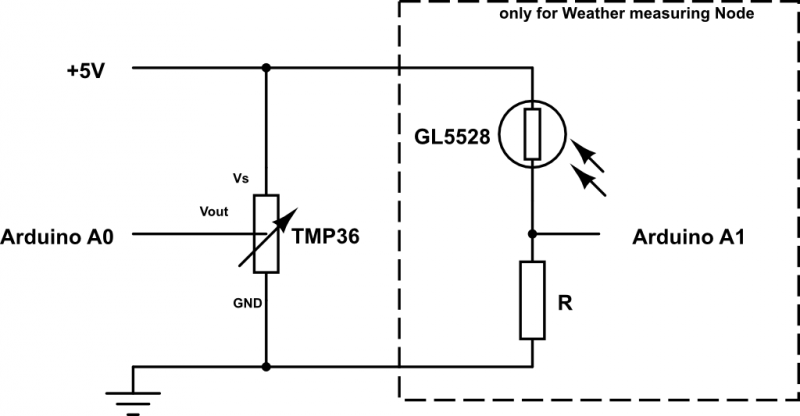
\includegraphics[width=0.75\textwidth]{../Images/Circuit.png}
\end{figure}
The \textbf{TMP36} is directly connected to the Arduino's 5V Power source and GND, the output voltage of the \textbf{TMP36} is read on the A0 Analog Input of the Arduino.
\\\\
On the weather measuring Node the circuit is enlarged by the \textbf{GL5528 LDR}. The LDR is used in a voltage divider circuit. The Voltage of 5 Volt is being divided by the propordion of the resistances of the LDR and the fixed Resistor. This “proportional divided” voltage is supplied to the A1 Analog Input of the Arduino.

\subsubsection{Collecting Node}
The Collecting Node consists of an Arduino Ethernet Board (A simple Arduino with Ethernet Shield would also be possible). The Arduino Ethernet board is also extended with a Wireless Proto Shield and XBee Module to provide ZigBee connectivity. The Arduino Ethernet features a built in micro SD Card slot.

\subsection{Software Architecture}
\subsubsection{Messaging}
\textbf{ZigBee Network Setup}
\\\\
The ZigBee Network consists of three Nodes
\begin{itemize}
\item Pond measuring Node
\item Weather measuring Node
\item Collecting Node
\end{itemize}
The Collecting Node will act as the ZigBee Coordinator, so its XBee Module will have to be loaded with the coordinator Firmware. the two measuring Nodes will be either End-Nodes (which means low power consumption), or routers (which gives them the ability to extend the Networks Radius by routing). Since both measuring Nodes only communicate with the collecting Node (very simple star-network-configuration) no additional routing Nodes are necessary. Also making the measuring Nodes act as routers will increase the power consumption of the Nodes.
\\\\
So as long as both measuring Nodes are in reach of the collecting Node, it is best to stick to the end-device firmware for the measuring Nodes XBee modules, otherwise the routing firmware might enhance the networks reach.
\\\\
In our Project we are going to use the ZigBee Network standard. This means that we won't concern ourself with the lower layers of the protocol stack. Because we only work on the upper Layers (Application Layer), the choice of firmware for the measuring Nodes is not relevant for our Software. ZigBee will take care that our packages get to their destination, either directly or via hopping the other measuring Node.
\\\\
In order to work with the XBee Modules we will use the xbee-arduino Library:\\ \url{http://code.google.com/p/xbee-arduino/}
\\\\
The XBee Modules are connected to the Arduino over a Serial Connection. The protocol to control the XBee Modules over the Serial connection is pretty easy, however the Library makes it even easier.
\\\\
Every XBee Module comes with a 64 Bit long Serial number that is also used as its own ZigBee Network Adress. The coordinator must know the adresses of the two measuring Nodes. It is possible for the Collector to discover the other Nodes using broadcasts, however we are going to hardcode the Meaurement Nodes adresses into the collectors Sourcecode. The Measuring Nodes are going to adress the collector either by taking its adress from the collectors packets, or by using the reserved Adress 0x0000000000000000 (coordinators 64 Bit adress).
\\\\
There is also a 16 Bit PAN (Personal Area Network) Adress that has to be set up on all Nodes. The exact adress is irellevant (as long as its 16 Bit long and the same on every Node). The Adress we are using will be dec 56154 = 0xDB5A. By the way, this adress was chosen by multiplying 42 by 1337.
\newpage
\textbf{ZigBee Network Messages}
\\\\
Between the Measuring Nodes and the Collector there are two Messages that have to be defined. The first there is the Measurements Request that the Collector sends to the Measuring Nodes. The second Message is the answer from the Measuring Nodes to the collector.
\\\\
Packages in the ZigBee Network transfer a payload of a certain number of bytes. In the Arduino language the payload would be an array of the type uint8\_ t.
\\\\
The following Messages with their specified structure are going to be transfered:\\\\
\textbf{Measurement Request}
\begin{table}[h]
    \begin{tabular}{|l|l|l|}
    \hline
    \rowcolor{dunkelgrau}
    Byte(s) & content  & meaning                            \\ \hline
    1       & 'R'=0x52 & identifier for Measurement Request \\ \hline
    \end{tabular}
\end{table}\\
1 Byte consisting of the uppercase letter 'R', indicating that this is a measurment request from the collector.
\\\\
\textbf{Weather Nodes Measurement Response}
\begin{table}[h]
    \begin{tabular}{|l|l|l|}
    \hline
    \rowcolor{dunkelgrau}
    Byte(s) & content  & meaning                                      \\ \hline
    1       & 'W'=0x57 & identifier for Measurement response          \\ \hline
    2-5     & float    & float for temperature measurement in Celsius \\
    6-9     & float    & float for light intensity in Lux             \\
    \end{tabular}
\end{table}\\
The first Byte indicates that this message is a measurement response from the Weather Measuring Node. The next 4 Bytes contain a float value of the measured temperature. The last 4 Bytes are are a float value for the measures light intensity.
\\\\
\textbf{Pond Nodes Measurement Response}
\begin{table}[h]
    \begin{tabular}{|l|l|l|}
    \hline
    \rowcolor{dunkelgrau}
    Byte(s) & content  		& meaning                            \\ \hline
    1       & ''P'= 0x50 	& identifier for Pond measuremnt response \\ \hline
    2-5		& float			& float for temperature measurement in Celsius \\ \hline
    \end{tabular}
\end{table}\\
The first Byte indicates that this is a measurement response from the Pond Measuring Node. The next four bytes contain a float value for the measured temperature in Celsius.
\\\\
\textbf{Communication between the Collector and the Application}\\\\
The Collector is hosting a TCP Server (static ip Adress and portnumber, hardcoded into sourcecode). The Application is going to connect to the collector as a client. After the TCP 3-Way handshake id over the collector is immediately going to transfer its CSV-File over the TCP conection to the Application. After the complete File is transfered the connection is being closed.

\newpage
\subsubsection{Collecting Node}
\textbf{CSV File Format:}
\\\\
The Data Collecting Node will store a CSV-File (Coma Seperated Values) on a SD Card. Every half an hour the collecting Node will require measurements from the measuring Nodes. The Measuring Nodes then adds a Line to the CSV-File. Also the PC Application will require the collecting Node to send the CSV-File over Ethernet. Each Line represents a complete measurement of the whole System.
\\\\
The Lines will have the following form:
\\\\
hh,mm,ss,dd,mm,yyyy,ppppp,aaaa,llll
\begin{itemize}
\item \textbf{hh, mm, ss, dd, mm, yyyy} represent the point in time when the measurements were taken.
\item \textbf{ppppp} is the temperature of the pond in \degree Celsius in the form of 12.5 meaning +12.5\degree C
\item \textbf{aaaaa} is the air temperature in \degree Celsius and is coded in the same way as the Pond's temperature
\item \textbf{llll} is the light level in Lux
\end{itemize}
In principle all values can be signed floating point numbers of arbitrary length, however only certain subsets of the possible values make sense. hh will be integer and of the interval [0 - 23]. mm and ss will be integer and of the interval [0-59]. For the temperatures float values from -30 to +45\degree C are realistic. Negative values get marked by a -. Unknown values might be left out, but the necessary comas will stay.
\\\\
Example Line:
\\\\
00,30,15,13,05,2013,11.5,9.7,
\\\\
At 0:30h and 15 seconds on the 13th of May of 2013, the pond temperature was 11.5\degree C, the air temperature was 9.7\degree C, and the lightlevel is unknown. The Lines will be seperated by a Newline '\textbackslash n'.
\\\\
In this Format, for every complete measurement, a line size of approximately 34 Bytes will be written to the File. Based on this Line Size the following estimations on Filesize can be made:
\begin{itemize}
\item 1 Measurement = 34 Bytes
\item 1 Day of measurements = 48 * 34 Bytes = 1632 Bytes
\item 1 Month of measurements = 31 * 1632 Bytes = 50.592 Bytes
\item 1 Year of measurements = 12 * 50.592 Bytes = 607.104 Bytes $\approx$ 593 kByte
\end{itemize}
With just a 32MB sized SD Card this System could collect Data for about 55 years. Since we will hardly be able to find an SD-Card of a size lower than 1GB it is obvious that Filesize is not going to be a problem.
\newpage
\textbf{Software Components:}
\\\\
Since the Collecting Node has several responsibilities in respect to functionality, it's Software consists of several Components:
\begin{figure}[h!]
  \caption{Collecting Node}
  \centering
    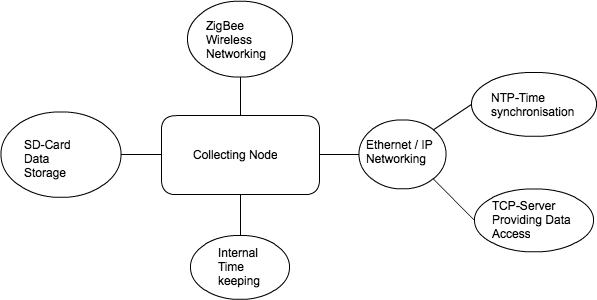
\includegraphics[width=0.75\textwidth]{../Images/collector_software_components.png}
\end{figure}
Those components get realised in the Software by writing so called Arduino Libraries. The Arduino Plattform provides several Libraries for different Services, but it also allows users to write their own Libraries. User defined Libraries get implemented by defining C++ classes that get instanciated in the Arduino sketch. This means that Arduino Libraries are just a way of using object oriented software development to modularize Arduino Sketches.
\\\\
The ZigBee Wireless Networking component takes care of everything the Collector has to do on the ZigBee Network, meaning to Send Measurement Requests and to receive the Measurement Responses from the Measuring Nodes. The Ethernet Networking component provides everything that has to be done using the Ethernet/IP Network connection. There are two functionalities provided by this component. First is the possibility to get the current Daytime and Date from a NTP Server. The second functionality is the hosting of a TCP Server, waiting for incomming connections. As a connection gets established the component sends the Data, which is stored using the SD-Data storage component, to the connected TCP-client (Our WSN-Accessing Application).
\\\\
The Component for intrnaly keeping the current Time and Date is not coded by us. It is the openly available Time Library by Michael Margolis. It uses the Arduino's internal function millis(), so no additional Hardware is needed to keep the time. The Time can be set by retrieving the UNIX standard Time (seconds since the 1st of January, 1970 00:00:00) and providing it to the Time library. It is then possible to retrieve the current Time in Hours, minutes and Seconds, as well as the calender date.
\\\\
The last component is the SD-Data storage component. It provides access to the SD-Card that can be inserted into a socket on the Arduino Ethernet board. On the SD-Card, there is one File created called “data.csv”. The SD-component adds CSV-Lines to the File, and can retrieve the File byte-wise.
\\\\
\textbf{Application Flow}\\\\
Arduino Sketches are always based on two core functions, setup() and loop(). Setup() contains all code that should run when the Arduino Board powers on, and loop() contains all the code that will run repeatedly until the Board gets powered off.
\\\\
Besides a lot of general initilization, inside setup() the collector does two things:
\begin{itemize}
\item Synchronize the Time using NTP
\item Create data.csv on the SD-Card if not present
\end{itemize}
For the operation of the Collector it is absolutely necessary to know the current Time and Date, thats why the collector first synchronizes using NTP. Then the data storage File gets created. If the file is already present, it will just be opened. The File does never get deleted by the collector!
\newpage
In the loop() function the collector works according to the following Algorithm:
\begin{figure}[h!]
  \caption{Collecting Node Flow Chart}
  \centering
    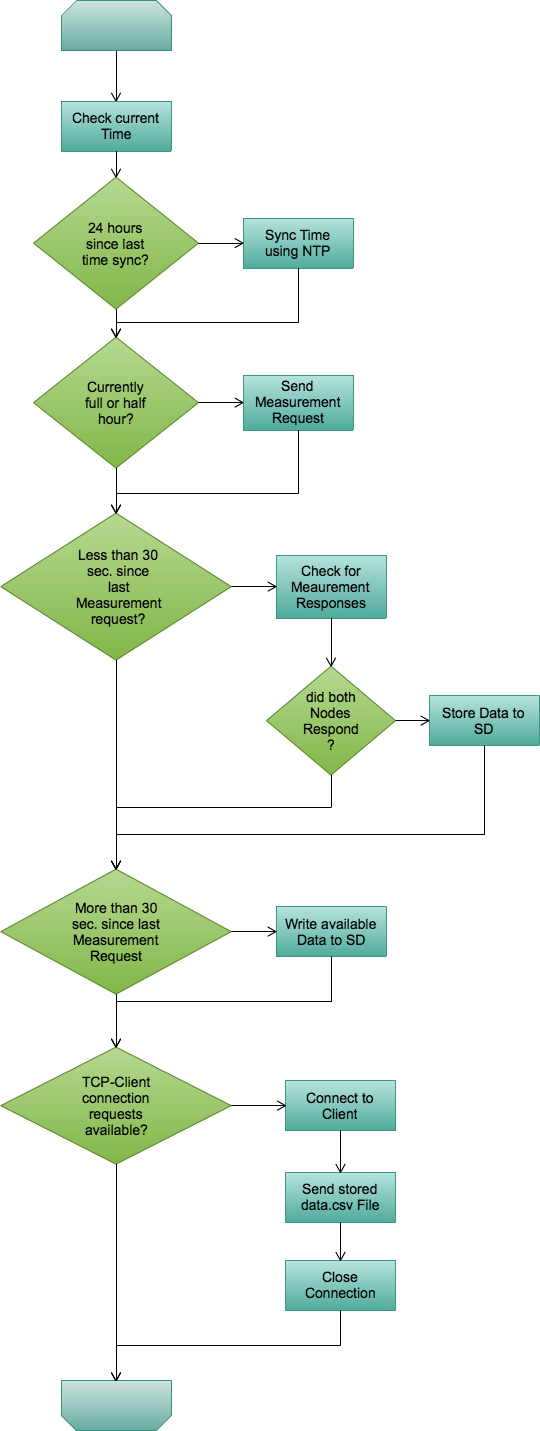
\includegraphics[width=0.45\textwidth]{../Images/collector_flow_chart.png}
\end{figure}

\subsubsection{Measuring Nodes}
The Measuring Nodes are seperated into two Parts. One Measuring Node measures Light and Temperature as an Weather Station outside. The other Measuring Node collect the temperature of a pond. The measured data is send via a tx package in the ZigBee Network to the Collector Node. Inside the Measuring Nodes there are executing following Functions:
\begin{itemize}
\item read Voltage from Analog Pin
\item Calculate Temperature 
\item Calculate Light
\item Send Temperature and Light Values via payload in a TX packet to Collector
\end{itemize}
\begin{figure}[h!]
  \caption{Measuring Nodes: Flow Chart}
  \centering
    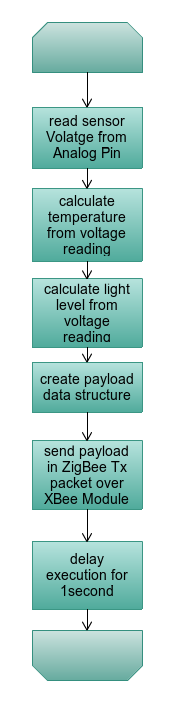
\includegraphics[width=0.20\textwidth]{../Images/Seq_Measuring.png}
\end{figure}
The Flow Chart shows, that the Measuring Nodes has a linear sequence of functions. These functions were repeated again and send temperature data and light data via a tx packet to the Collector Node.

\subsubsection{Application}
The features of the Application are described in the list of requirements. To imagine how the application behaves and how to modularize it we begin by creating a mock-up of the GUI:
\begin{figure}[h!]
  \caption{Mock-Up: Application}
  \centering
    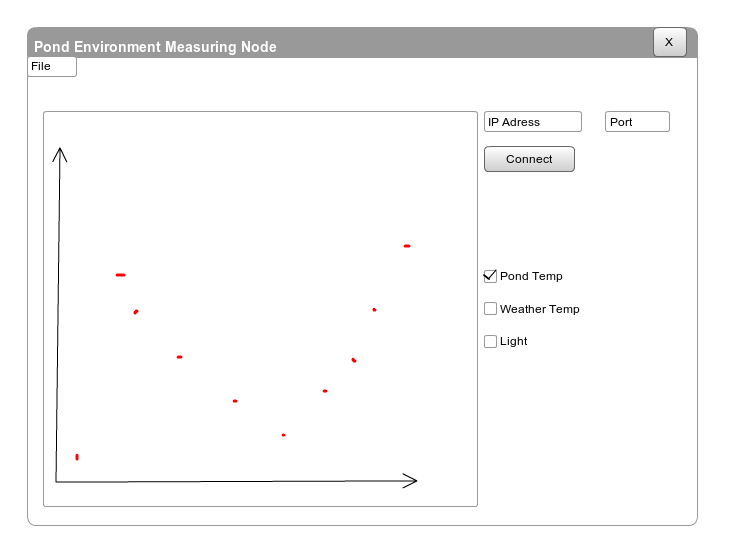
\includegraphics[width=0.75\textwidth]{../Images/Application.png}
\end{figure}
This is the graphical user Interface. On the left side is a \textbf{plotting area} where the history of measured Data is shown as a plot. On the right side are some necessary controlls.
\\\\
First there are two \textbf{input boxes} where the IP Adress and Port number, to reach the Collecting Node's TCP Server, are specified. After this input is made the connection can be established by clicking the \textbf{connect button}. If the connection fails an error dialog box will pop up, if it works the application will receive the CSV File's contents as byte stream (maybe show a progress bar dialog) and store it in local memory. After that the Data is being processed and plottet in the \textbf{plotting area}.
\\\\
On the right side are also three \textbf{check boxes} to select the values to be plottet. So by selecting the checks, curves are being drawn or removed from the \textbf{plotting area}. The curves are drawn in different colors so that they are distinguishable.
\\\\
On top of the GUI is a \textbf{menue bar} with a menue \textbf{“file”}. This menue only contains the entry \textbf{“Export as CSV”}. On selection of this entry a “save file” Dialog will pop up which allows to save the CSV files contents in a CSV-File on the PC's hard drive (like a copy of the CSV File on the Collecting Node).
\\\\
The Software Architecture follows the MVC Pattern and has the components shown in the following Graphic:
\begin{figure}[h!]
  \caption{Application-Architecture}
  \centering
    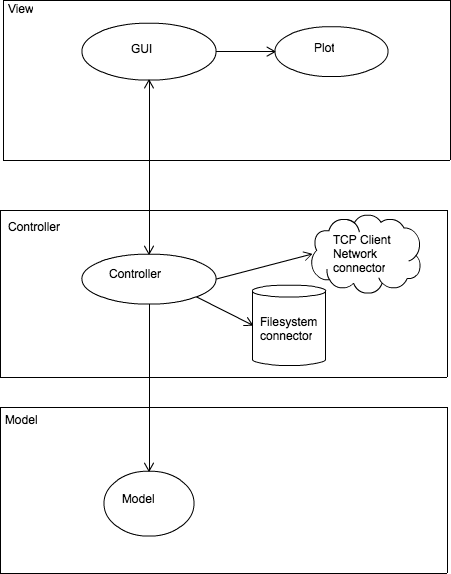
\includegraphics[width=0.50\textwidth]{../Images/application_architecture.png}
\end{figure}


% -------------------------- Project Estimation --------------------------------------
\newpage
\section{Project Estimates}
\subsection{Estimation technique Function Point}
Function Point Estimation was developed by A.J. Albrecht of t he IBM Corporation in the early 1980s. 
\\
The idea behind Function Points is to identify and quantify functionality required for a project. This procedure is decomposed into three parts:
\begin{enumerate}
\item Defining the Unadjusted Function Point Count
\item Determining the Value Adjustment Factor
\item Determining Function Points
\end{enumerate}
\textbf{Defining the Unadjusted Function Point Count}\\\\
\begin{figure}[h!]
  \caption{Function Point Model}
  \centering
    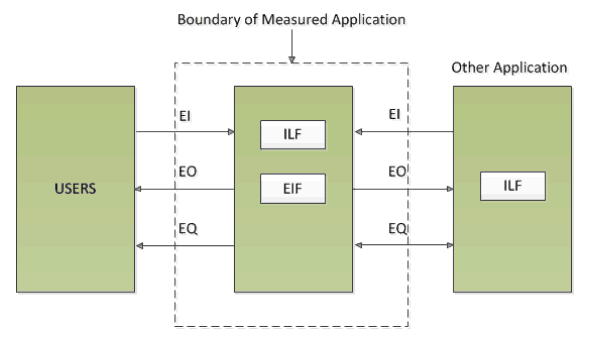
\includegraphics[width=0.5\textwidth]{../Images/FP_model.png}
\end{figure}
The application boundary defines what is external to the application. The number of Unadjusted Function Points is derived from the number and complexity of transactions functionalities like:
\begin{itemize}
\item \textbf{External Inputs (EI)} which are elementary processes (an elementary process is the smallest unit of activity that is meaningful to the user) in which data crosses the boundary from outside of the application. They come from input screens or other applications.
\item \textbf{External Outputs (EO)} which are elementary processes in which derived data passes across from inside to outside.  These screens, reports, graphs, messages are created from one or more logical files and external interface files.
\item \textbf{External Queries (EQ)} which are processes with both input and output components that  result in data retrieval from one or more internal logical files and external files.
\end{itemize}
and data functionalities like:
\begin{itemize}
\item \textbf{Internal Logical Files (ILF)} which are user groups of logically related data that reside within the application boundary. They are maintained through external inputs.
\item \textbf{External Interface Files (EIF)} which are user groups of logically related data that are use for reference only.
\end{itemize}
Using above data we can calculate the Unadjusted Function Points. After having all basic data and transactional functionalities of the system we can use the following table below to calculate.
\begin{figure}[h!]
  \caption{Unadjusted Function Point Count and Multipliers (Degree of Complexity)}
  \centering
    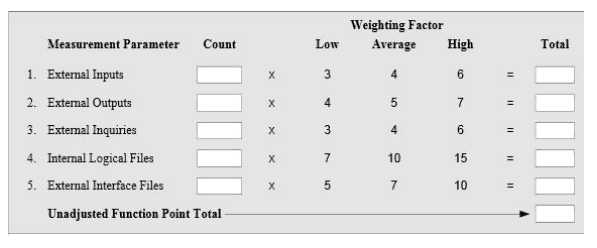
\includegraphics[width=0.75\textwidth]{../Images/FP.png}
\end{figure}\\\\
\textbf{Determining the Value Adjustment Factor}\\\\
Further we can calculate the Value Adjustment Factor based on 14 general system characteristics:

\begin{tabular}{ll}
 \parbox{8cm}{
 \begin{enumerate}
	\item Data Communication Complexity
	\item Distributed Data Processing Complexity
	\item Performance Complexity
	\item Heavily Used Configuration Complexity
	\item Transaction Rate Complexity
	\item On-line Data Entry Complexity
	\item End-User efficiency Complexity
 \end{enumerate}}
 &
 \parbox{7.5cm}{
 \begin{enumerate}
	\item On-Line Update Complexity
	\item Complex processing Complexity
	\item Reusability Complexity
	\item Installation Ease Complexity
	\item Operational Ease Complexity
	\item Multiple Sites Complexity
	\item Facilitate Change Complexity
 \end{enumerate}}
\end{tabular}

\begin{figure}[h!]
  \caption{Total Degree of Influence)}
  \centering
    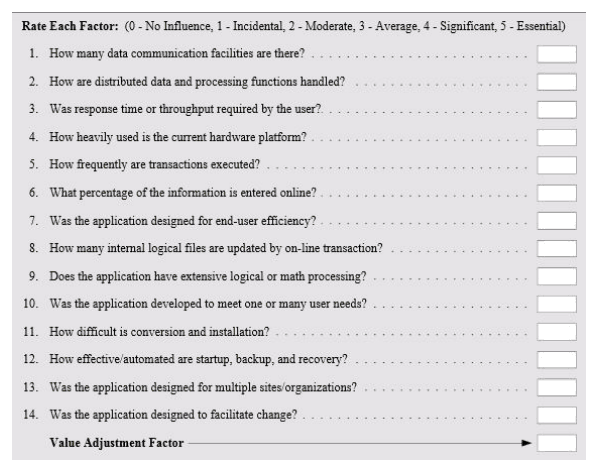
\includegraphics[width=0.75\textwidth]{../Images/FP_2.png}
\end{figure}
The general system characteristics are estimated on a scale of  0 to 5 (Degree of Influence)\\
\textbf{Total Degree of Influence = Sum of Degree of Influence}
\\\\
\textbf{Determining Function Points}\\\\
Determining Function Points consists of factoring Unadjusted Function Points and Value Adjustment Factor together.\\
\textbf{Value Adjustment Factor = 0.65 + (0.01 x Total Degree of Influence)}\\
\textbf{Function Points  = Unadjusted Function Points x Value Adjustment Factor}\\\\
Example 1: How long will a project take?\\
Let us assume we have:
\begin{itemize}
\item Unadjusted Function Points = 22
\item Value Adjustment Factor = 0,84
\item Function Points: 22 x 0,84 = 18,48
\end{itemize}
Here is a table, which shows a general Function Point estimation:\\\\
\begin{tabular}{|l|l|l|}
\hline
    \rowcolor{dunkelgrau}
	Project & Function Points 	& Man-Months 	\\ \hline
	ASD 	& 11 				& 1				\\ \hline
	KWO 	& 24 				& 2				\\ \hline
	RMD 	& 53 				& 5				\\ \hline
	WBO 	& 72 				& 6				\\ \hline
\end{tabular}\\\\
Having a look at an organization project benchmark we estimate a result of 1.5 Man-Months. At the end of our project we do have in effect an actual amount of 1.2 Man-Months which we then update in our organization estimation chart.\\\\
\begin{tabular}{|l|l|l|}
\hline
    \rowcolor{dunkelgrau}
	Project & Function Points 	& Man-Months 	\\ \hline
	ASD 	& 11 				& 1				\\ \hline
	Arduino	& 22				& 1.2			\\ \hline
	KWO 	& 24 				& 2				\\ \hline
	RMD 	& 53 				& 5				\\ \hline
	WBO 	& 72 				& 6				\\ \hline
\end{tabular}\\\\
Effort in Person Month = FP divided by number of FP per month (Using an organization or industry benchmark)\\
The Programmers in a company average 18 FP per month.\\
197 FP / 18 FP = 11 Man- Months


% ------------------------------- Project Schedule ---------------------------------
\section{Project Schedule}
Look at ../Gantt/ProjectPlan.pdf

% -------------------------------- Staff Organization ----------------------------
\section{Staff Organization}
\subsection{Team structure}
The team is organized without any hierarchically behaviors, all team members are equal. The members are:
\begin{itemize}
	\item Alexander K. - knoetig@stud.fh-frankfurt.de
	\item Sabrina B. - sabrina.bajorat@gmail.com
	\item Rozana A. - rozanamail1@yahoo.com
	\item Alexander V.D. - vallejodirektor@googlemail.com
\end{itemize}The Team Members had following Tasks:
\begin{itemize}
	\item Alexander K. - Documentation, Wiki Administrator, Implementation of Collecting Node and Application (GUI, TestServer)
	
	\item Sabrina B. - Documentation, Project Plan, Gantt Chart, Implementation of Measuring Nodes and Application (GUI, TestServer)

	\item Rozana A. - Domain Expert (Arduino, Xbee)

	\item Alexander V.D. - Estimation of Project
\end{itemize}

\subsection{Management reporting and communication}
There are every week status reports of done and open tasks for the current and next week. The main organization and communctions follows over the Wiki (\url{http://vs1164102.vserver.de/dokuwiki/doku.php?id=ssns:ssns-project}).


% -------------------------------- Project Results ------------------------------
\section{Project Results}
According to our Architecture Designs we started to implement our assigned software products. Since the technology of Arduino and XBee was new to us, implementation followed the principles of trial and error, with a lot of experimental coding. It was difficult for us to estimate the complexity of the task to implement the software according to the planned architecture. At some points we had to do some cutbacks to the requirements to finish the product in time. Unfortunatelly we were unable to get the Wireless Sensor Network to work. The main reason for that is that we were unable to get the collecting Nodes Software to work.
\\
In the following sections we describe what we have archieved in respect to the software components.


\subsection{Software for the Collecting Node}

The Collecting Node was the most complex Software component, and unfortunatelly it was not finished in time. Alexander Knötig was the developer responsible for that component.
\\\\
As planned in the Architecture design, the collecting Nodes Software consists of several components implementing subtasks of the collecting Node. Only the components for handling the SD-Card access and the handling of Time and Date have been working as supposed. The components responsible for ZigBee Network connectivity and Ethernet connectivity could not be made working. The problem with implementing those components (and all the other components as well) is related to the Arduino Development Environment.
\\\\
It is made to be simple and easy to learn for programming beginners. But those simplififications also enforce limitations on the programmer. For example, there is no real control over which object files get linked together in order to resolve dependencies. This is especially problematic when writing libraries (like the components of the collecting Node) that use other libraries. The header files of used Libraries always get included, so the necessary files can get compiled, but when trying to link them together, the necessary object files from the libryries don't get linked. There are workarounds to this problem, but they tend to make the code hard to work with.
\\\\
Another limitation of the Arduino Development environment is the missing possibility to debug the code. Professional Development Environments for microcontrollers (Like Atmels ATmega) provide possibilities to debug the software while it is running on the microcontroller. This is offcourse more complex that debugging Software for usual PC Operating Systems, but it is a possibility to understand what is going wrong. When using Arduino, it is not possible to see what is running wrong. You can upload your programm to the board and then observe the results, either the board does what it is supposed to be doing, or it doesn't. There are no Exception Messages (like in Java programms), no hex Dumps, and not even a sign if the microcontroller has shut down because of a severe error. If the Arduino Board encounters an error while executing the programm code it just stops the programms execution. There is no possibility to see where it crashed and why.
\\\\
When trying to implement the Collecting Node we often encountert the sutiation that the software just did not work, but we were unable to find out why. Thats why we were unable to finish it in time.


\subsection{Software for the Measurement Nodes}

The Softwar for the Measurement Nodes was relatively simple, relative to the collecting nodes Software. But since the collecting Node was not working, it was also not possible to operate the measurement Nodes with it together. The Mesuring Nodes are supposed to be waiting for a Measurement Request Message from the Collecting Node, when receiving this request, the Measuring Nodes send an Response Message.
\\\\
Because of the missing Collecting Node, we were unable to implement the concept of waiting for an request and answering with an response. Instead, we implemented the measuring Nodes to periodically send a response Message, without listening for Requests.


\subsection{WSN Accessing Application}

The WSN Accessing Application was supposed to feature a Table and a Graph to visualize the Data that was going to be read in from the Collecting Node. But over the course of the project we changed the applications features a little bit. But the core function of reading the csv file from the Collecting Node and saving it to the computers hard drive is left unchainged. The implemented Application features a textarea displaying the loaded csv file as it is, and also two graphs, one for plotting the curve of the lightlevel and one for plotting two curves for the temperature measurements.

% -------------------------------- Protocol -------------------------------------
\newpage
\section{Protocol}
\begin{tabular}{ll}
 \parbox{8cm}{
 %%% Week 16 ---------------------------------------------------------------------
\large{\textbf{Week 16}}
\begin{itemize}
\item Team Formation
\item Resarch of Hardware (Arduino, XBee)
\end{itemize}
%%% Week 17 ---------------------------------------------------------------------
\large{\textbf{Week 17}}
\begin{itemize}
\item Research of Hardware
\item Collecting Project Ideas
\item Experiments with Arduino
\end{itemize}
%%% Week 18 ---------------------------------------------------------------------
\large{\textbf{Week 18}}
\begin{itemize}
\item Decision on Project Goal
\item Project Specification
\item Requirement Analysis
\item Experiments with Arduino
\end{itemize}
%%% Week 19 ---------------------------------------------------------------------
\large{\textbf{Week 19}}
\begin{itemize}
\item Requirement Analysis
\item Project Plan
\item Create Circuit-Design
\end{itemize}
%%% Week 20 ---------------------------------------------------------------------
\large{\textbf{Week 20}}
\begin{itemize}
\item Project Plan Version 1
\item Create Circuits
\end{itemize}
}
 &
 \parbox{8cm}{
%%% Week 21 ---------------------------------------------------------------------
\large{\textbf{Week 21}}
\begin{itemize}
\item Create System Architecture: Hardware Architecture
\item Continue with Project Plan
\end{itemize}
%%% Week 22 ---------------------------------------------------------------------
\large{\textbf{Week 22}}
\begin{itemize}
\item Create System Architecture: Software Architecture
\item Implementation of Collecting and Measuring Nodes
\item Continue with Project Plan 
\end{itemize}
%%% Week 23-25 ---------------------------------------------------------------------
\large{\textbf{Week 23-25}}
\begin{itemize}
\item Implementation of ZigBee Network
\item Implementation of Application TestServer + Graphical View of measured data
\item Continue with Project Plan 
\end{itemize}
%%% Week 26-27
\large{\textbf{Week 26-27}}
\begin{itemize}
\item Test Software
\item Finish Project Plan
\item Prepare Presentation
\end{itemize}
 }
\end{tabular}

% ---------------------------------------------------------------------------------------
\newpage
\begin{thebibliography}{9}
\bibitem{}Arduino Library {\url{http://arduino.cc/en/Reference/Libraries}}
\bibitem{}Arduino XBee Library {\url{https://code.google.com/p/xbee-arduino/}}
\bibitem{}XBee {\url{http://www.digi.com/xbee/}}
\bibitem{}XBee {\url{http://xbee.wikispaces.com/}}
\bibitem{}TMP36 {\url{http://www.analog.com/static/imported-files/data_sheets/TMP35_36_37.pdf}}
\bibitem{}GL5528 {\url{https://www.sparkfun.com/datasheets/Sensors/Imaging/SEN-09088-datasheet.pdf}}
\bibitem{}{\url{http://www.pjrc.com/teensy/td_libs_Time.html}}
\bibitem{Faludi}Building Wireless Sensor Networks: With ZigBee, XBee, Arduino, and Processing", Robert Faludi, O'Reilly Media; Auflage: 1 (31. Januar 2011)
\bibitem{Conell}Mc Connell, Rapid Development, Microsoft Press, 1996
\bibitem{Jones}C. Jones, Applied Software Measurement, 1991, McGraw Hill
\bibitem{Garmus}D. Garmus and D. Herron, Measuring the Software Process, Prentice Hall, 1996
\bibitem{Balzert}Helmut Balzert, Lehrbuch der Software-Technik, Spektrum Akademischer Verlag 2001
\end{thebibliography}
\end{document}